%%%%%%%%%%%%%%%%%%%%%%%%%%%%%%%%%%%%%%%%%%%%%%%%%%%%%%
\chapter{Datasets}
\label{datasets}
\graphicspath{{chapter_03/figures}{chapter_03/tables}}
%%%%%%%%%%%%%%%%%%%%%%%%%%%%%%%%%%%%%%%%%%%%%%%%%%%%%%



To develop accurate and reliable flash flood prediction models, it is essential to consider various parameters that influence flash flood occurrence, such as rainfall, soil moisture, vegetation type, and the slope of the orography, among others. This thesis will use such parameters for short- and medium-range forecasts from the ERA5 reanalysis computed at ECMWF.

The ERA5 reanalysis offers a spatially and temporally consistent and high-quality reconstruction of past atmospheric and land surface conditions, crucial for training data-driven models. However, the spatial resolution of rainfall from ERA5 (\textasciitilde31 km) is not sufficiently high for flash flood applications. Hence, the ecPoint post-processing technique is employed in this thesis to address the limitations of the coarse spatial resolution of the raw rainfall ERA5 short- and long-range forecasts. The ecPoint methodology uses a decision-tree-based algorithm to anticipate sub-grid variability and correct biases in the raw NWP model outputs, producing probabilistic point-scale rainfall predictions that are more skilful and reliable against point verification, especially in the case of extreme localised rainfall. Such characteristics make ERA5-ecPoint rainfall short- and medium-range forecasts better suited for flash flood applications. 

Extensive observational records of flash flood impacts play a crucial role in developing and validating the data-driven flash flood prediction model. Global impact models exist, such as EM-DAT and DesInventar. However, they largely underrepresented flash flood frequency due to their event inclusion protocols and not uniform spatial coverage around the world \citep{Panwar_2020}. This thesis will, therefore, use a higher-density regional flash flood impact database developed in the US, the Storm Event Database. 

The \marginpara{Chapter structure} remainder of this chapter is structured as follows. \textbf{Section 2} focuses on the raw datasets used in this research, namely the ECMWF Ensemble Forecasts and the ERA5 Reanalysis, and it provides an overview of their characteristics. The verification of the raw datasets will be discussed together with the post-processed data in Section 3. \textbf{Section 3} is divided into three subsections: \textit{section 3.1} describing the ecPoint post-processing method, including the calibration process, creation of forecasts and reanalysis, and computational requirements; \textit{section 3.2} presents the verification of ensemble and ecPoint rainfall forecasts; and \textbf{section 3.3} discusses the verification of ERA5 and ecPoint-ERA5 data. \textbf{Section 4} presents the observational datasets used in this study: \textit{section 4.1} covers rainfall observations, and includes the description of the datasets, their spatial and temporal coverage, strengths, and limitations, data availability and gaps; \textit{section 4.2} covers flash flood impact observations from global databases such as EM-DAT and DesInventar, as well as higher-density national databases from the US and Ecuador, providing description of the datasets and their metadata, analysis of their spatial coverage and granularity to assess relevance in flash flood analysis, strengths and limitations. Finally, \textbf{Section 5} summarizes the key findings of the data chapter, highlighting the strengths and limitations of the datasets used, it discusses potential gaps in the current data landscape, and offers recommendations for future data collection and integration efforts in the field of flash flood prediction. 



%%%%%%%%%%%%%%%%%%%%%%
\section{Study domain}

This research establishes the CONUS as the primary study domain for the flash-flood-focused rainfall verification, data-driven model development, and predictability assessment of medium-range data-driven predictions of areas at risk of flash floods. The domain considered in this thesis in shown in Figure \ref{fig:conus_domain}. The selection of this geographical region is methodologically justified on several grounds. Foremost is the higher quality and comprehensiveness of the \textit{Storm Event Database} maintained by the National Oceanic and Atmospheric Administration (NOAA). 

\begin{figure}[htbp]
\centering
\includegraphics[scale=0.65]{01_conus_domain_orography.png}
\caption{\textbf{CONUS domain.} The figure shows the orography at 1 km resolution (in shades of green and brown) and the location of the 25 most populated cities (black dots) over the CONUS.}
\label{fig:conus_domain}
\end{figure}

This database systematically records flash flood occurrences with high spatial and temporal resolution, including crucial metadata regarding impact severity, affected areas, and casualty information. The database's consistent reporting protocols and rigorous quality control procedures mitigate the observational uncertainty that typically plagues flash flood research \citep{Panwar_2020}.

The CONUS domain further presents methodological advantages through its diverse hydro-meteorological conditions, encompassing varied topographical features ranging from coastal plains to mountainous terrain, and climatic regimes spanning Mediterranean, continental, subtropical, and desert classifications. This diversity enables the development of a machine learning model exposed to a broad spectrum of flash flood generating mechanisms, from intense convective precipitation to rain-on-snow events, thereby enhancing its potential transferability to global applications.

Whilst the primary model development utilises the CONUS domain, the global applicability of the methodology necessitates consideration of how domain-specific characteristics might influence model performance when transferred to regions with different hydro-climatological conditions. These considerations are addressed in subsequent sections detailing the global application of the flash flood prediction model.


%%%%%%%%%%%%%%%%%%%%%%%%%%%%%%%%%%%%%%%%%%%%%
\section{ERA5}

Short- and long-range ERA5 forecasts were acquired at their native resolution (\textasciitilde31 km at the equator), for a period covering the years 1950 to 2024. Table \ref{table:forecasts_types} describes the characteristics of both forecasts (e.g., spatial and temporal resolution, run times, and maximum lead time). The short-range forecasts (also known as "reanalysis") will be used to train the data-driven model. The long-range forecasts will be used to assess the predictability of the data-driven medium-range (i.e., up to day 5) predictions of the areas at risk of flash floods.

\begin{table}[htbp]
\centering
\captionof{table}{\textbf{ERA5 short- and long-range forecasts.} The table describes the characteristics of short- and long-range forecasts from ERA5.}
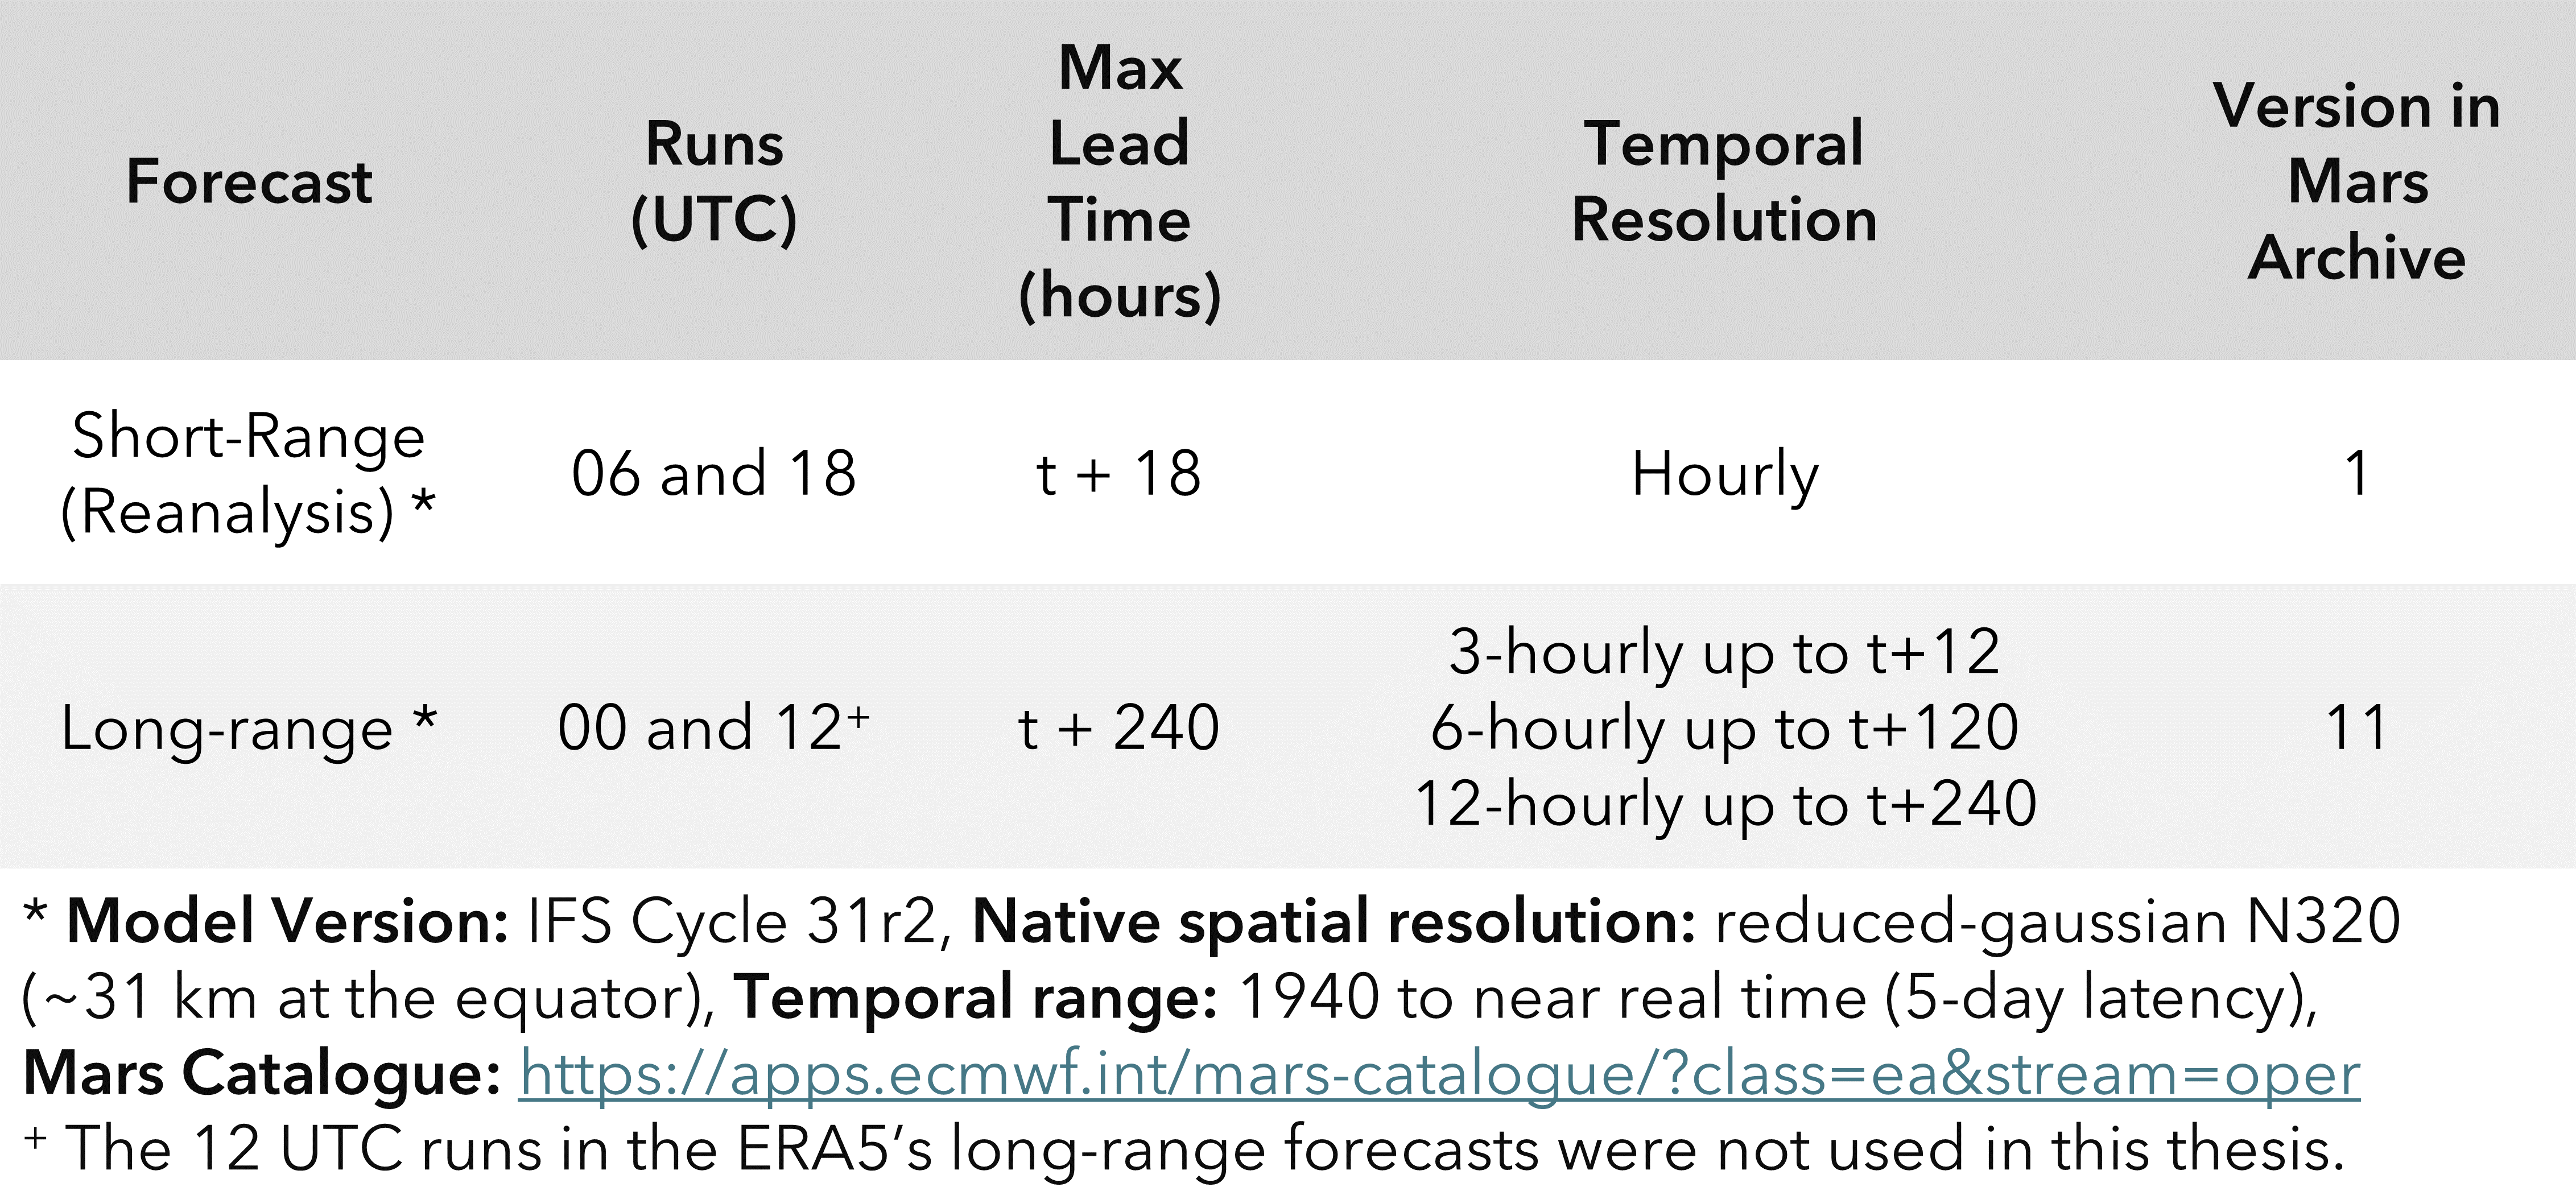
\includegraphics[width=\textwidth]{01_forecasts_types.png}
\label{table:forecasts_types}
\end{table}

From the extensive suite of variables included in ERA5\footnote {The full set of parameters included in the short- and long-range forecasts from ERA5 can be found in the Mars Catalogue at \url{https://apps.ecmwf.int/mars-catalogue/?class=ea&stream=oper}.}, the subset of dynamic and static parameters listed in Table \ref{table:parameters_used} were considered to compute those parameters whose relationship with flash flood occurrence has been established in previous literature, such antecedent soil moisture, slope of the orography, and vegetation. The following sub-sections describe the pre-processing of the raw ERA5 parameters to compute the variables that will be included in the data-driven model.

\begin{table}[htbp]
\centering
\captionof{table}{\textbf{Parameters used from ERA5 and ERA5-ecPoint.} Description of the parameters considered for developing the data-driven short- and medium-range predictions of areas at risk of flash floods over a continuous global domain.}
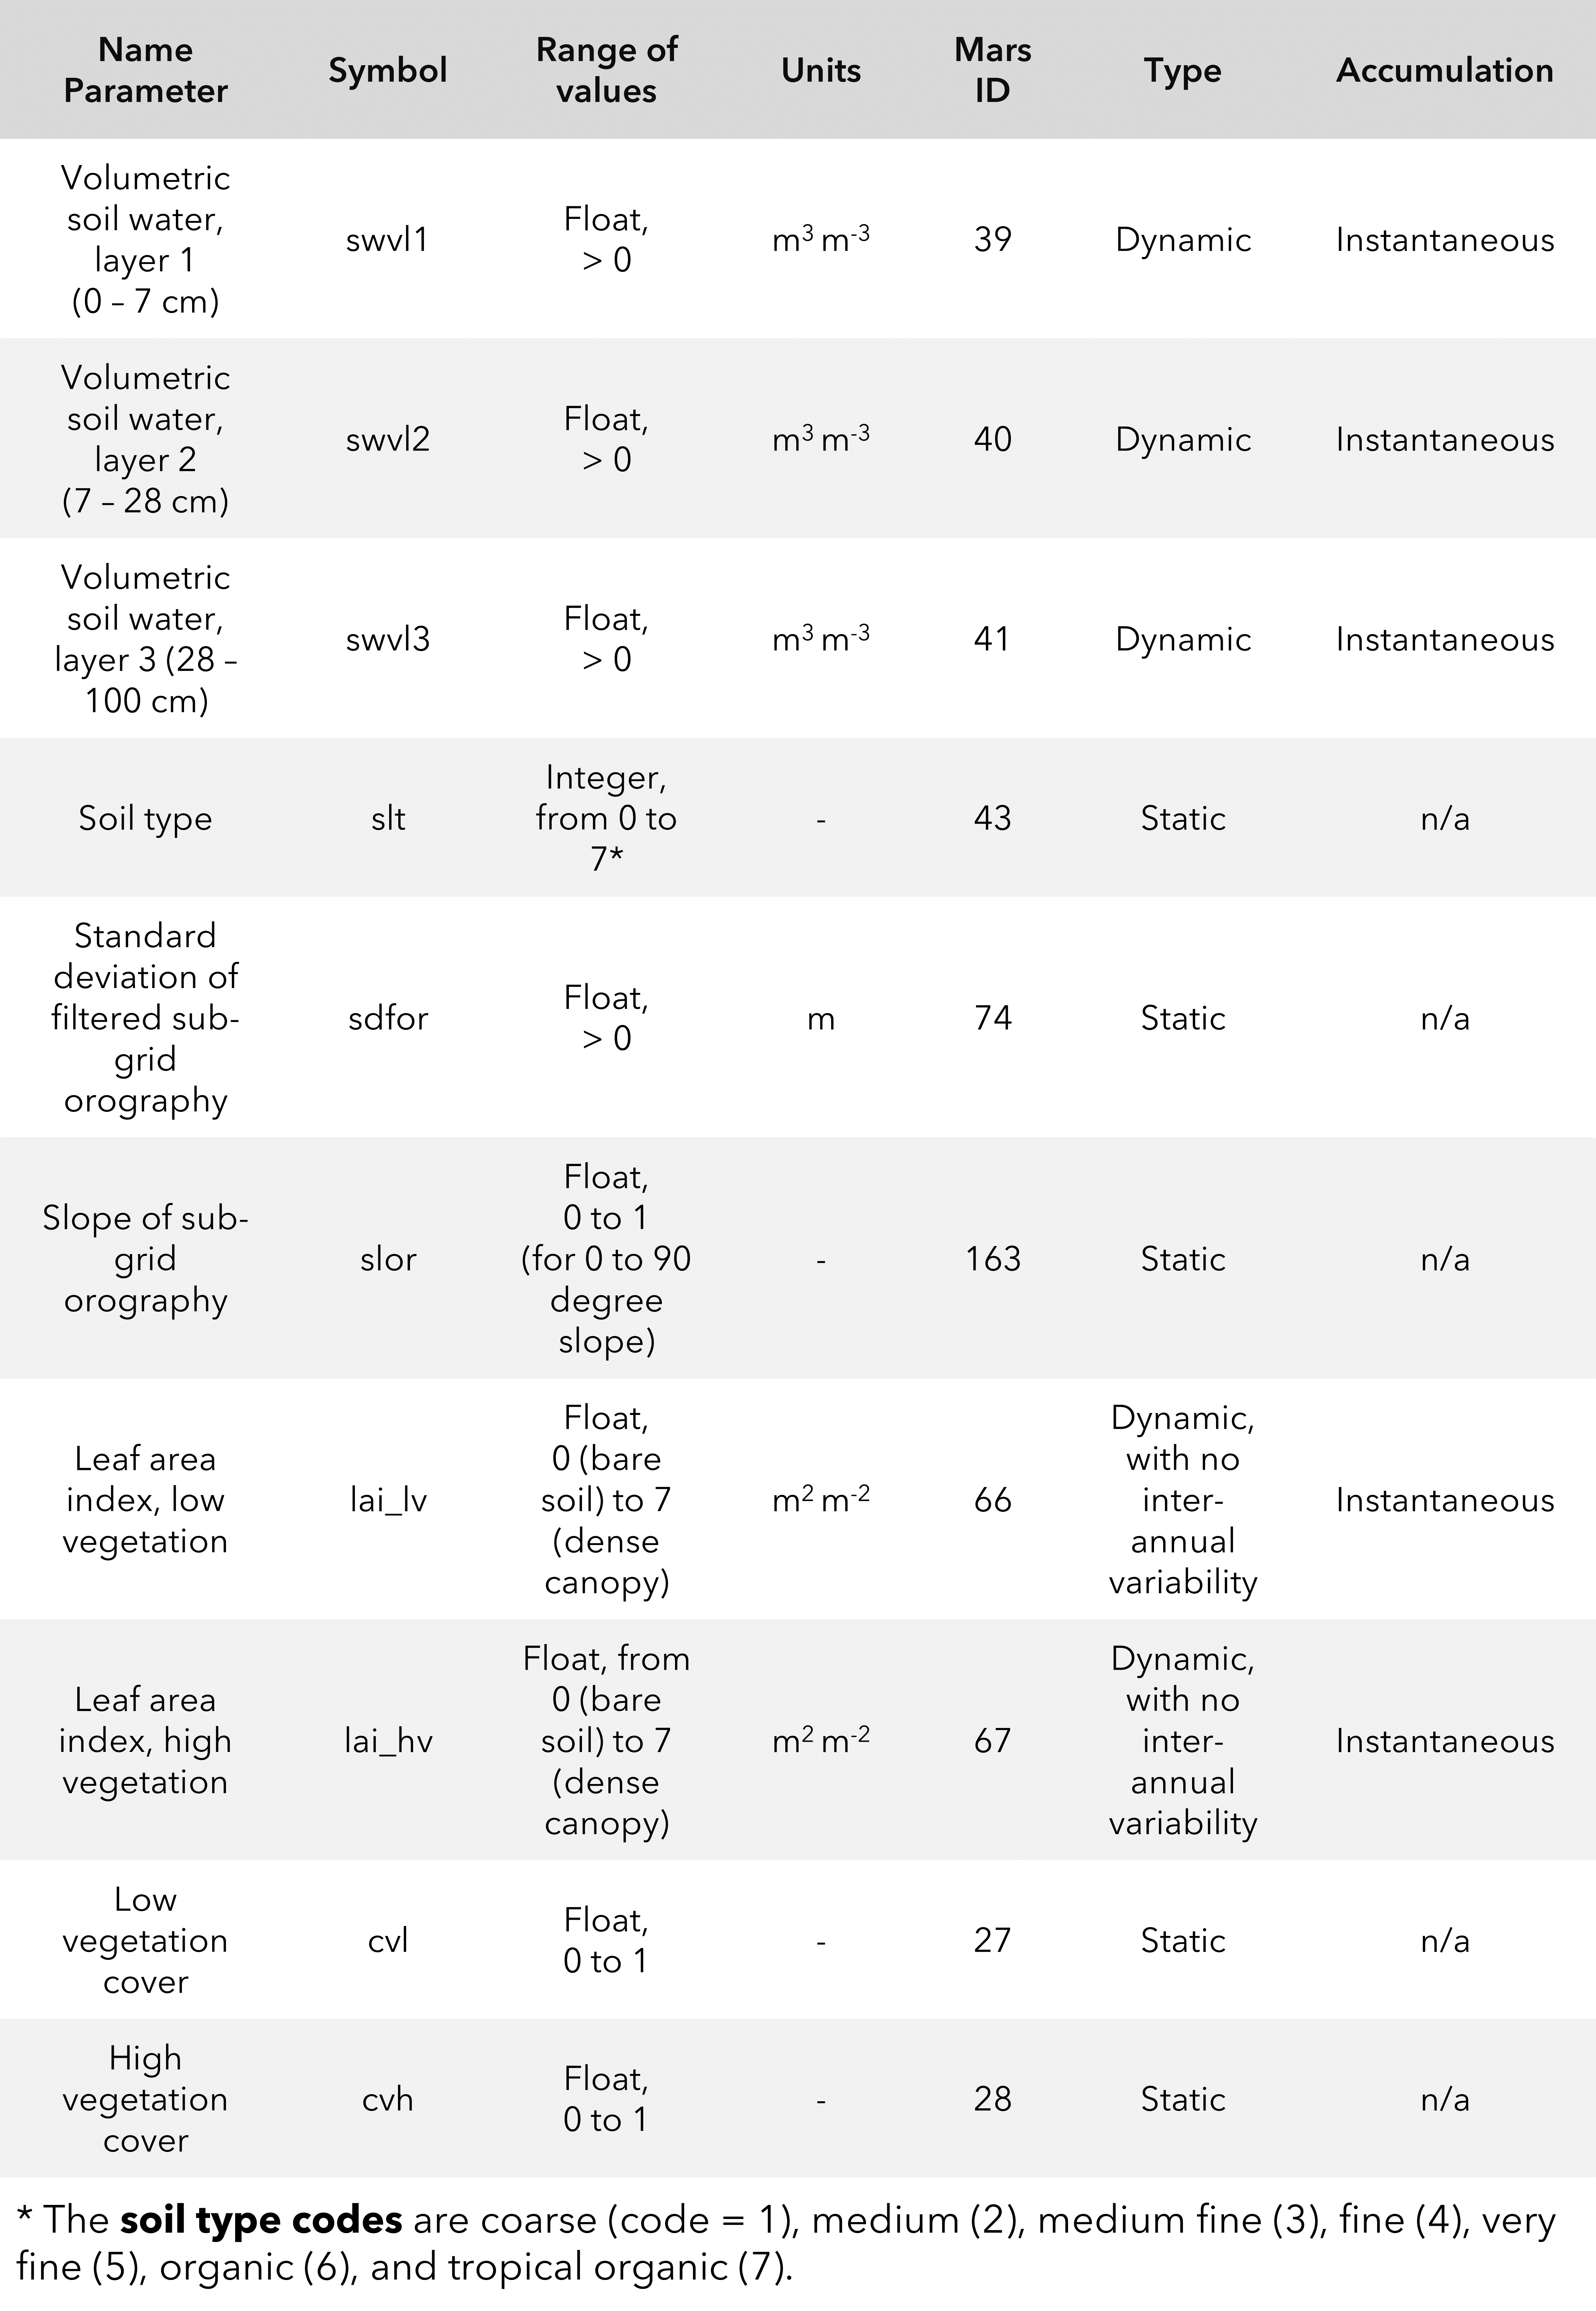
\includegraphics[width=\textwidth]{02_era5_params.png}
\label{table:parameters_used}
\end{table}


\subsection{Antecedent soil moisture}

For antecedent soil water content, this study considers the percentage of soil maximum saturation in the top 1 m layer of soil, 24 hours prior to a flash-flood-triggering rainfall event. The percentage of soil maximum saturation in the top 1 m of soil is computed considering the pre-established values of maximum soil saturation for different types of soil, and integrating those over layers 1, 2, and 3 of the volumetric soil water. Table \ref{max_saturation} shows the pre-defined values of maximum soil saturation used at ECMWF for different types of soil \citep{Balsamo_2009}:

\begin{table}[htbp]
\centering
\captionof{table}{\textbf{Maximum saturation} The table shows the pre-defined values of maximum soil saturation per soil type used at ECMWF \citep{Balsamo_2009}.}
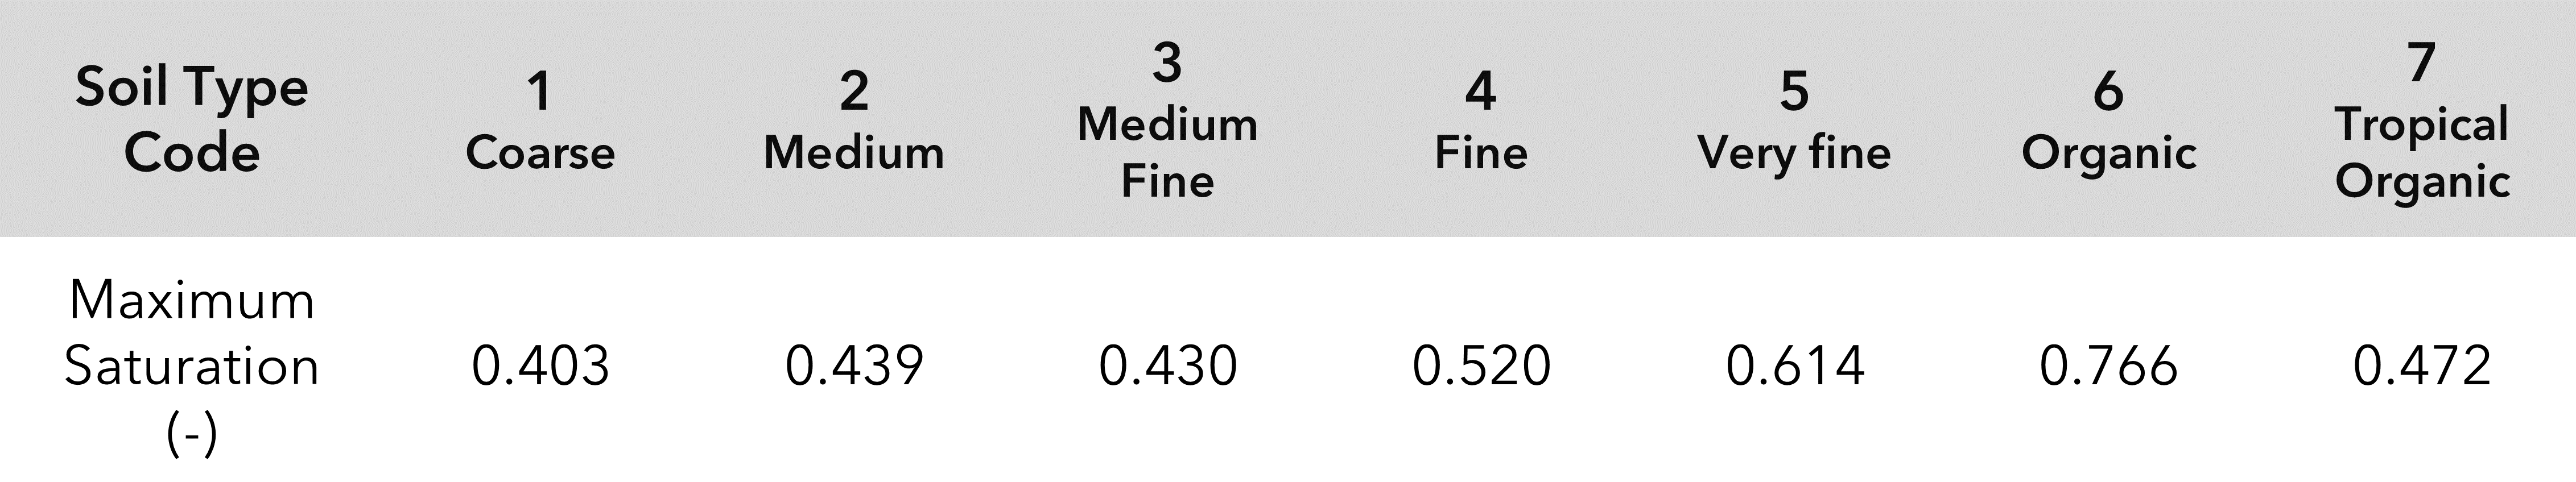
\includegraphics[width=\textwidth]{03_max_saturation.png}
\label{table:max_saturation}
\end{table}

Equations \ref{eq:max_sat_field} and \ref{eq:indicator} show how the fields containing the percentage of soil saturation were computed. 

\begin{align}
\text{max\_sat\_field}
  &= \sum_{i=01}^{N} \text{max\_sat}_i \,\mathbf{1}_{\{s=c_i\}}
     \label{eq:max_sat_field}\\
\mathbf{1}_{\{s=c_i\}}
  &=
  \begin{cases}
    1, & s=c_i,\\
    0, & s\neq c_i.
  \end{cases}
    \label{eq:indicator}
\end{align}

where, N goes from 1 to 7, and it represents the codes for the soil type.

Equation \ref{eq:swvl} computes the soil water content over the top 1m layer of the soil:

\begin{equation}
\label{eq:swvl}
\text{swvl} = \sum_{j=1}^{M} \text{swvl}_{j}\, \text{depth}_{j}
\end{equation}

where, M goes from 1 to 3, and it represents the soil layers.

Finally, equation \ref{eq:swvl_perc} computes the percentage of soil saturation:

\begin{equation}
\label{eq:swvl_perc}
\text{swvl\_perc} = \frac{\text{swvl}}{\text{max\_sat\_field}}
\end{equation}

Figure \ref{fig:perc_soil_saturation_sr} shows a map plot for the percentage of soil saturation.

\begin{figure}[htbp]
\centering
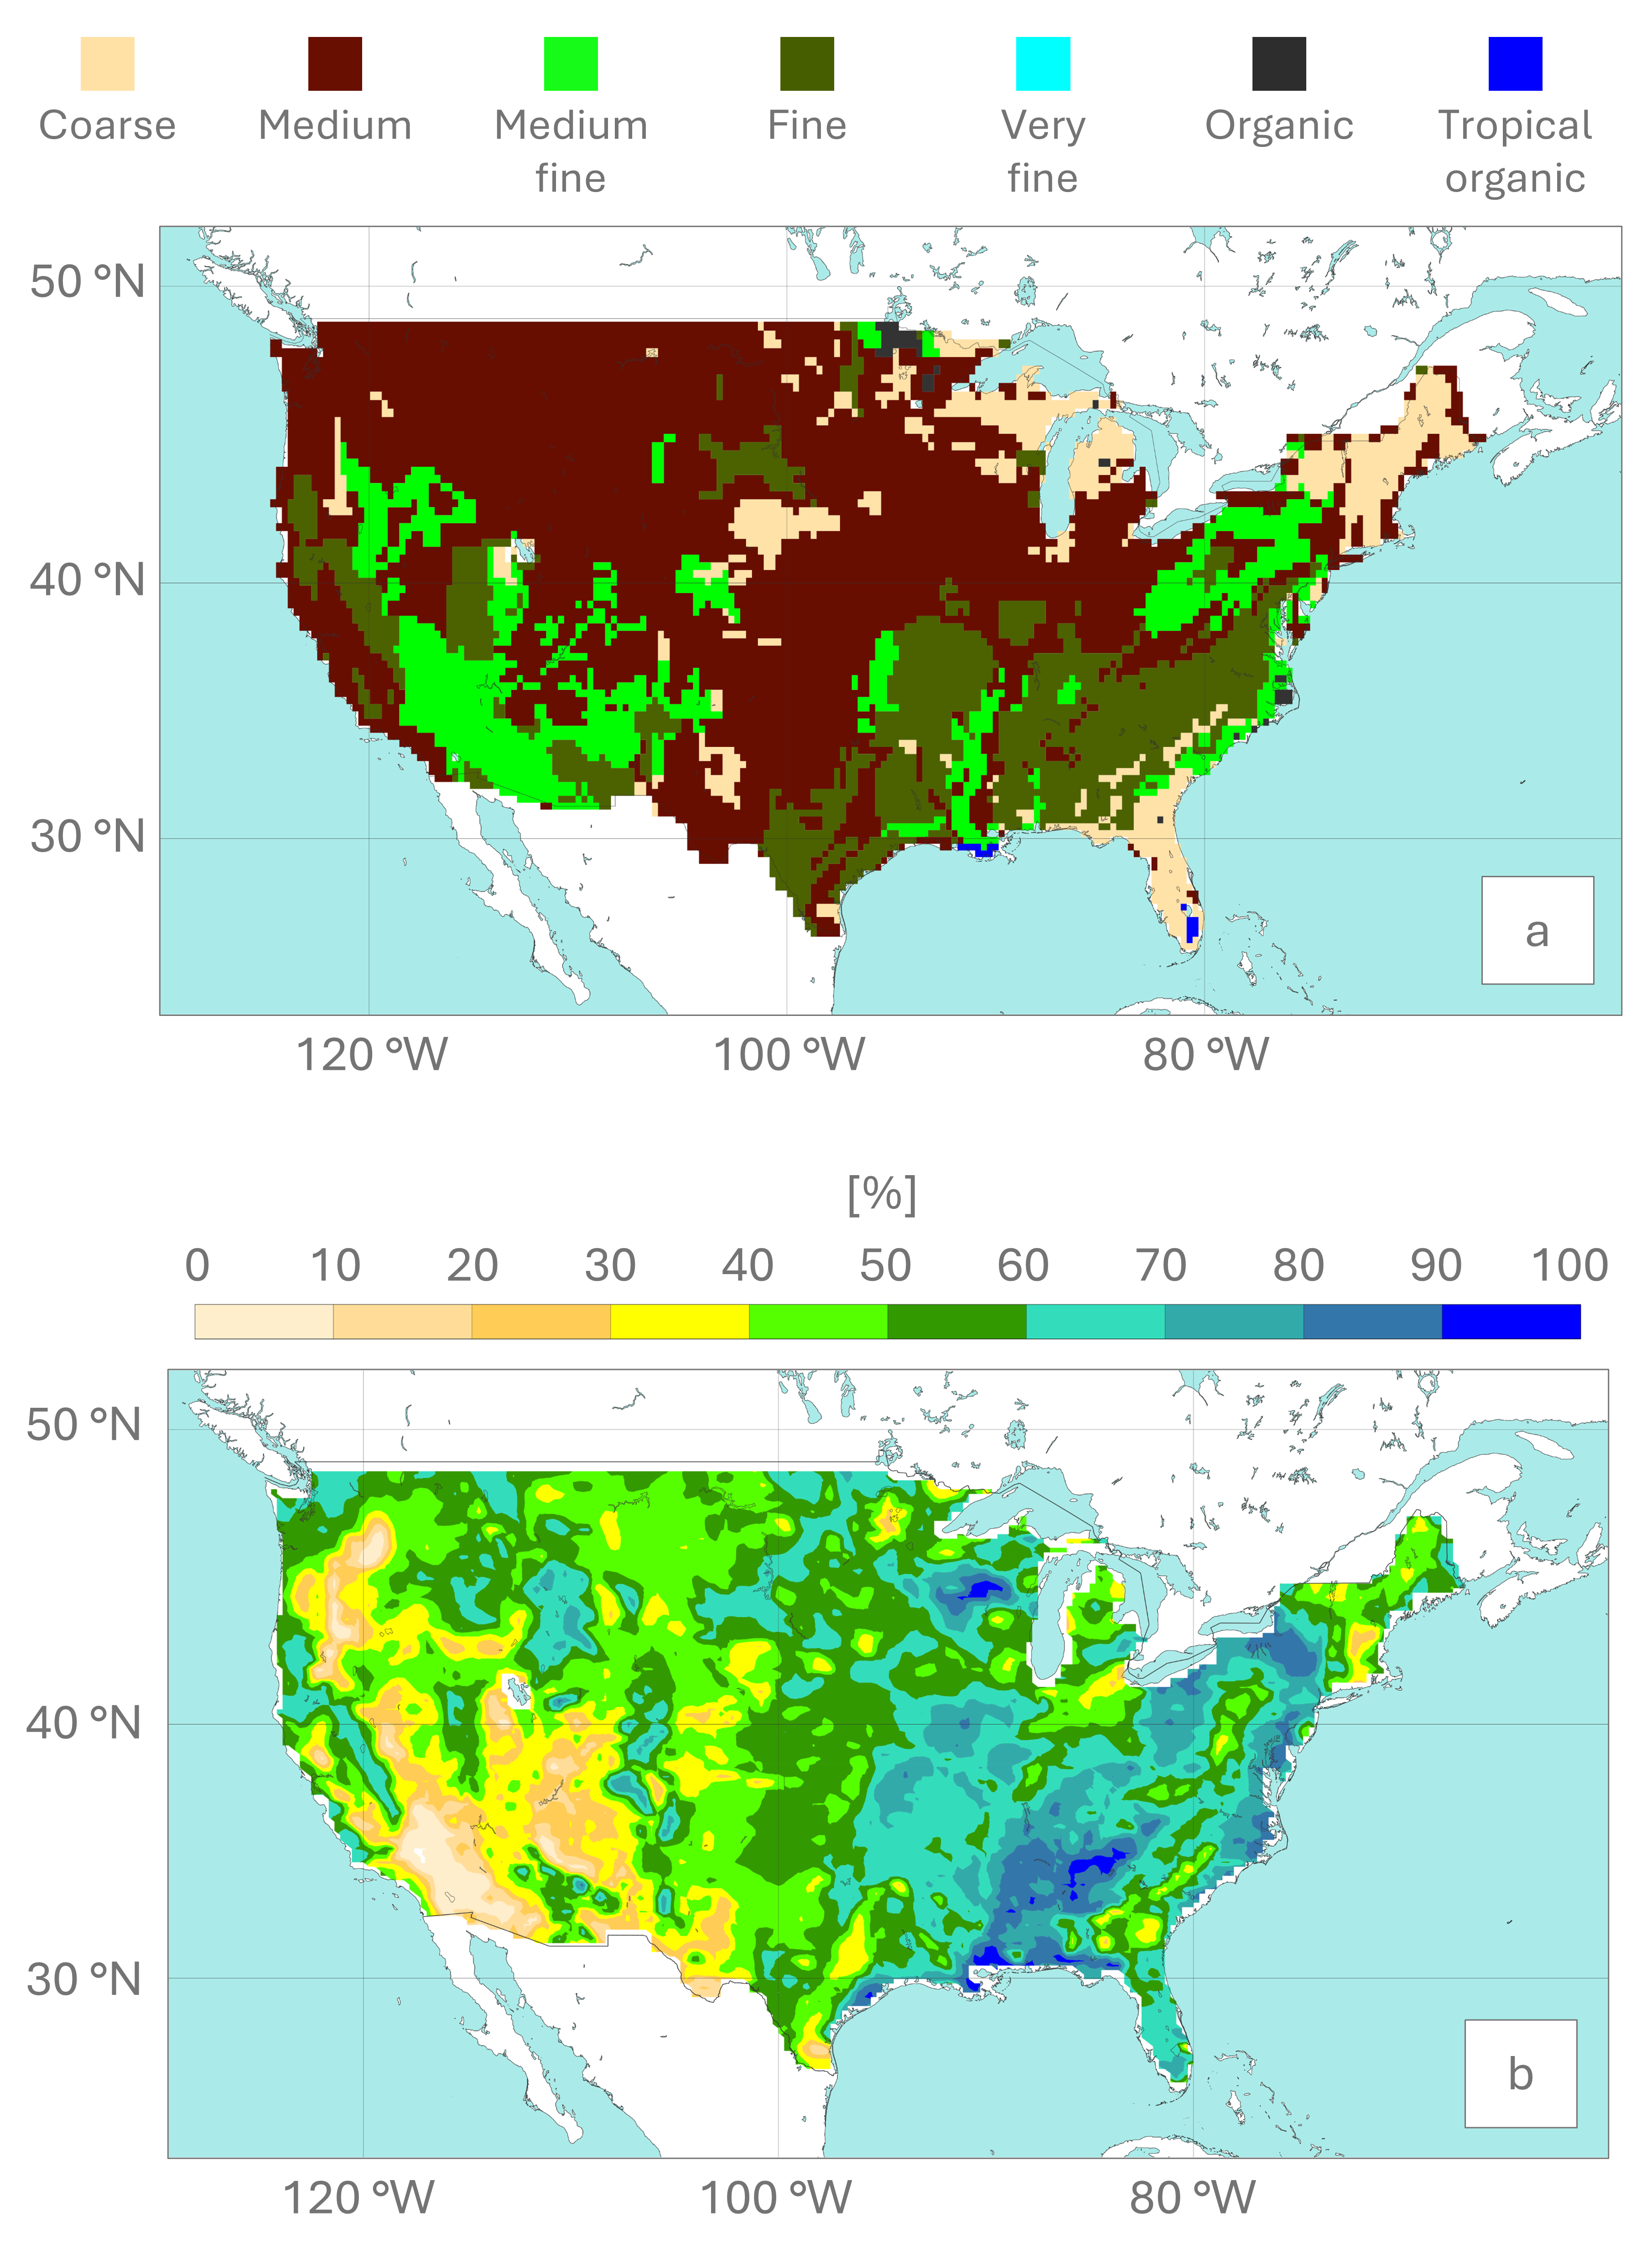
\includegraphics[width=\textwidth]{03_perc_soil_saturation_sr.png}
\caption{\textbf{Percentage of soil saturation} Panel (a) shows the spatial distribution over the CONUS of the soil type categories in ERA5. Panel (b) shows an example of the percentage of soil saturation for the short-range ERA5 for a VT between 31-08-2021 12 UTC and 01-09-2021 00 UTC.}
\label{fig:perc_soil_saturation_sr}
\end{figure}


\subsection{Parameters to represent orography}




\subsection{Vegetation}

The leaf area index (LAI) is obtained from the ERA5 monthly averaged data on single levels. It is obtained by combining the variables called “leaf area index, high vegetation” and “leaf area index, low vegetation” on a per-grid-cell basis using the fractions of high and low vegetation prescribed in the model, respectively known as high vegetation cover and low vegetation cover.




24-hourly flash flood outlooks were considered, and hence accumulated or instantaneous variables were considered accordingly for the correspondent 24 hourly flash flood outlooks.





%%%%%%%%%%%%%%%%%%%%%%%%%%%%%%%%%%%%%%
\section{Post-processed rainfall data}

While ERA5 provides a comprenhensive suite of hydro-meteorological variables, its native precipitations output echibits known limitations in representing rainfall's sub-grid variability, which is crucial for flash flood prediction.To adress this limitation, this study employs ERA5-ecPoint, a post-processed rainfall forecast that enhances the representation of point-scale rainfall totals within each grid-box.  

\subsection{The ecPoint post-processing method}

\subsubsection{Calibration process}

\subsubsection{Creation of ecPoint-based forecasts and reanalysis}

\subsubsection{Computational requirements}


\subsection{Verification of ecPoint Rainfall forecasts}


\subsection{Verification of ecPoint-ERA5}



%%%%%%%%%%%%%%%%%%%%%%%%%%%%%%%%%%%%%%%%%%%%%%%%%%%%%%%%%%%%%%%%%%%%%%%%%%
\section{Flash flood impact observations: Storm Event Database over CONUS}
\label{storm_event_database}

\subsection{Dataset Description}

The NOAA National Centers for Environmental Information (NCEI) Storm Event Database serves as the US's official repository of severe weather records, including flash floods. This comprehensive database has evolved significantly since its inception in 1950, transforming from county-level tornado reports to a sophisticated system documenting up to 48 different weather phenomena with increasingly precise geospatial representation. For flash flood research and machine learning applications, understanding the database's structure, evolution, and limitations is essential for robust methodology development. 

The NCEI Storm Event Database began in 1950 as a limited collection focusing primarily on tornado documentation, and since then, the database has undergone significant expansion. Until 1954, it recorded only tornado events, while from 1955 to 1995, its coverage expanded to include tornadoes, thunderstorm winds, and hail events. From 1996, the database expanded to contain a comprehensive documentation of 48 distinct event types, including flash floods\footnote{\url{https://www.ncdc.noaa.gov/stormevents/details.jsp}}. 

This historical progression affects data completeness for different phenomena. Flash flood records only became standardised from 1996 onward, with major geographical precision improvements implemented in 2007 when reporting transitioned from county-level to polygon-based representation\footnote{\url{https://inside.nssl.noaa.gov/flash/database/}}.

The database covers the entire United States and territories with a spatial bounding box from 172.0°W to 65.0°E longitude and 18.0°N to 72.0°N latitude\footnote{\url{https://www.ncei.noaa.gov/access/metadata/landing-page/bin/iso?id=gov.noaa.ncdc:C00510}}. Data collection involves a network of 123 NWS Forecast Offices gathering information from emergency management officials, law enforcement, trained SKYWARN spotters, damage surveys, media reports, and public observations\footnote{\url{https://www.ncdc.noaa.gov/stormevents/faq.jsp}}.

In this study, we are using version 3.1 of the database, we consider only reports over the CONUS that go from 2001 to 2024.


\subsection{Metadata Quality}

The Storm Event provides extensive metadata for flash flood events. Among all the available keys, we considered in this study only the keys described in table 3





Although professional meteorologists and hydrologists collect flash flood reports to include in the Severe Storm Database, any human augmented reporting system is subject to variations in population density, diurnal cycles of human activity, and more mundane transcription or memory errors that affect the timing and location of reports \citep{Barthold_2015}. Evidence of these issues has been found in assessments of FFG skill \citep{Clark_2014}, and it has been found that the distribution of SED's flash floods reports is affected by the distribution of human population \cite{Marjerison_2016}. 



\subsection{Coverage, Granularity, and Relevance for Flash Flood Analysis}

\subsection{Strengths and Limitations}


































%%%%%%%%%%%%%%%%%%%%%%%%%%%%%%%%%%%%%%%
\section{Summary and recommendations}

\subsubsection{Dataset Summary}

\subsubsection{Data Gaps and Limitations}

\subsubsection{Future Recommendations}